
% part 20
\section{Колеса внутри колес: Twisted и Erlang\label{sec:part20}}

\subsection{Введение}

%One fact we’ve uncovered in this series is that mixing synchronous “plain Python” code with asynchronous Twisted code is not a straightforward task, since blocking for an indeterminate amount of time in a Twisted program will eliminate many of the benefits you are trying to achieve using the asynchronous model.
Один факт, который мы еще не рассмотрели это то, что смешивание 
обычного синхронного Python кода с асинхронным Twisted кодом - задача 
непростая, поскольку блокирование на непродолжительный период времени в 
Twisted программе может испортить все то, что 
вы пытались достичь, используя асинхронную модель.   


%If this is your first introduction to asynchronous programming it may seem as if the knowledge you have gained is of somewhat limited applicability. You can use these new techniques inside of Twisted, but not in the much larger world of general Python code. And when working with Twisted, you are generally limited to libraries written specifically for use as part of a Twisted program, at least if you want to call them directly from the thread running the reactor.
Если это ваше первое введение в асинхронное программирование, то 
может показаться, что приобретенное знание имеет ограниченную применимость.  
Вы можете использовать все эти новые техники внутри Twisted, 
но не в большинстве Python программ. При работе с Twisted, в основном, 
вы ограничены библиотеками, написанными специально для 
использования как части Twisted программы, поменьшей мере, 
если вы хотите их вызывать напрямую из потока, в котором 
запущен реактор.  


%But asynchronous programming techniques have been around for quite some time and are hardly confined to Twisted. There are in fact a startling number of asynchronous programming frameworks in Python alone. A bit of searching around will probably yield a couple dozen of them. They differ from Twisted in their details, but the basic ideas (asynchronous I/O, processing data in small chunks across multiple data streams) are the same. So if you need, or choose, to use an alternative framework you will already have a head start having learned Twisted.
Но техника асинхронного программирования используется много где и 
довольно давно и едва ли ограничена Twisted. Для Python'а существует 
много других асинхронных систем. Немного поискав, вы найдете достаточно 
много реализаций. Детально они отличаются от Twisted, но основные 
идеи (асинхронный ввод-вывод, обработка данных маленькими порциями среди 
множество потоков данных) остаются те же. Поэтому, если вам нужно 
использовать другую систему, то вы уже будете иметь преимущество, 
изучив Twisted.  


%And moving outside of Python, there are plenty of other languages and systems that are either based around, or make use of, the asynchronous programming model. Your knowledge of Twisted will continue to serve you as you explore the wider areas of this subject.
Перемещаясь за пределы Python'а, существует 
много других языков и систем, которые основаны или 
используют асинхронную модель программирования. Ваше 
знание Twisted будет служить вам при открытии более 
широкой области этого предмета.


%In this Part we’re going to take a very brief look at Erlang, a programming language and runtime system that makes extensive use of asynchronous programming concepts, but does so in a unique way. Please note this is not meant as a general introduction to Erlang. Rather, it is a short exploration of some of the ideas embedded in Erlang and how they connect with the ideas in Twisted. The basic theme is the knowledge you have gained learning Twisted can be applied when learning other technologies.
В этой главе мы очень коротко посмотрим на 
\href{http://erlang.org/}{Erlang}\footnote[1]{http://erlang.org/} -  
язык программирования и исполняющая система (runtime system), которая активно 
использует концепции асинхронного программирования, но делает 
это уникальным образом. Обратите внимание, что далее не следует  
общее введение в Erlang. Скорее, это короткое раскрытие некоторых 
идей, заложенных в Erlang, и как они связаны с идеями в Twisted. 
Основная тема - знания, которые вы приобрели, изучая Twisted, 
могут быть применены при изучении других технологий.



\subsection{Переосмысленные обратные вызовы}

%Consider Figure 6, a graphical representation of a callback. The principle callback in Poetry Client 3.0, introduced in Part 6, and all subsequent poetry clients is the dataReceived method. That callback is invoked each time we get a bit more poetry from one of the poetry servers we have connected to.
Рассмотрим графическое 
представление обратного вызова (callback) на рисунке \ref{fig:reactor-callback}. Основной callback в 
поэтической 
\href{http://github.com/jdavisp3/twisted-intro/blob/master/twisted-client-3/get-poetry.py#L1}{клиенте 3.0}, 
представленном в главе \ref{sec:part6}, и во всех 
последующих поэтических клиентах - метод 
\href{http://github.com/jdavisp3/twisted-intro/blob/master/twisted-client-3/get-poetry.py#L56}{dataReceived}. 
Этот callback вызывается каждый раз, когда мы получаем 
часть поэзии из поэтических серверов, к которым мы 
присоединились.


%Let’s say our client is downloading three poems from three different servers. Looking at things from the point of view of the reactor (and that’s the viewpoint we’ve emphasized the most in this series), we’ve got a single big loop which makes one or more callbacks each time it goes around. See Figure 40:
Допустим, наш клиент скачивает три поэмы из трех 
различных серверов. Посмотрим на вещи с точки зрения 
реактора (на этой точки зрения мы акцентировали внимание 
во многих главах), мы имеем один большой цикл, который 
делает один или более обратных вызовов при каждой проходе. 
Посмотрим на рисунок \label{fig:reactor-2}. 

% fig40
\begin{figure}[h]
\begin{center}
    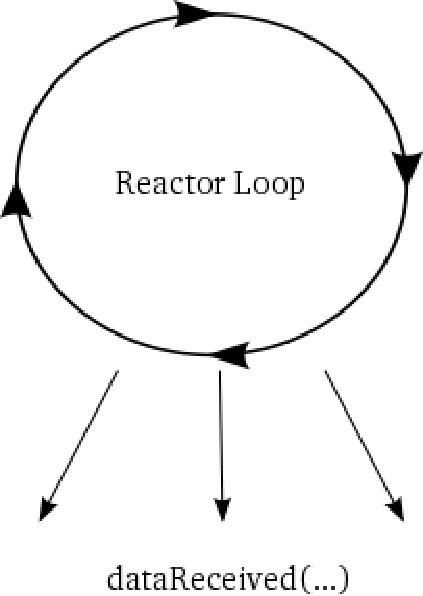
\includegraphics[height=0.3\textheight]{images/reactor-2.pdf}
    \caption{обратные вызовы с точки зрения реактора\label{fig:reactor-2}}
\end{center}
\end{figure}


%This figure shows the reactor happily spinning around, calling dataReceived as the poetry comes in. Each invocation of dataReceived is applied to one particular instance of our PoetryProtocol class. And we know there are three instances because we are downloading three poems (and so there must be three connections).
Этот рисунок показывает, что реактор успешно вращается 
вокруг, вызывая \textit{dataReceived} по приходу  поэзии. 
Каждый вызов \textit{dataReceived} применяется к одному из 
определенных экземпляров нашего класса \textit{PoetryProtocol}. 
И мы знаем, что существует три экземпляра, поскольку 
мы скачиваем три поэмы (и поэтому должно быть три соединения). 


%Let’s think about this picture from the point of view of one of those Protocol instances. Remember each Protocol is only concerned with a single connection (and thus a single poem). That instance “sees” a stream of method calls, each one bearing the next piece of the poem, like this:
Давайте думать о картинке с точки зрения одного 
из наших экземпляров Protocol. Этот экземпляр "видит" 
поток при вызове метода, который каждый раз
приносит следующую порцию поэмы:

\begin{scriptsize}\begin{verbatim}
dataReceived(self, "When I have fears")
dataReceived(self, " that I may cease to be")
dataReceived(self, "Before my pen has glea")
dataReceived(self, "n'd my teeming brain")
...
\end{verbatim}\end{scriptsize}

%While this isn’t strictly speaking an actual Python loop, we can conceptualize it as one:
Поскольку это похоже на цикл в Python'е, 
мы можем концептуализировать это так:

\begin{scriptsize}\begin{verbatim}
for data in poetry_stream(): # pseudo-code
    dataReceived(data)
\end{verbatim}\end{scriptsize}

%We can envision this “callback loop” in Figure 41:
Мы можем представить себе это "цикл обратных вызовов" на 
рисунке \ref{fig:callback-loop}.

% fig41
\begin{figure}[h]
\begin{center}
    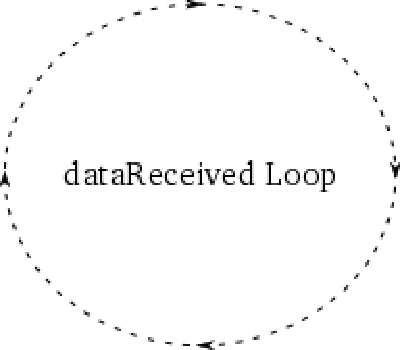
\includegraphics[height=0.3\textheight]{images/callback-loop.pdf}
    \caption{Виртуальный цикл обратные вызовов\label{fig:callback-loop}}
\end{center}
\end{figure}


%Again, this is not a for loop or a while loop. The only significant Python loop in our poetry clients is the reactor. But we can think of each Protocol as a virtual loop that ticks around once each time some poetry for that particular poem comes in. With that in mind we can re-imagine the entire client in Figure 42:
И снова, это не цикл \textit{for} и не цикл \textit{while}. 
Единственно существенным циклом в наших поэтических клиентах 
является реактор. Но мы можем думать о каждом Protocol'е, 
как о виртуальном цикле, который прокручивается каждый раз 
при появлении поэмы. Имея это в виду, мы можем представить 
заново весь клиент на рисунке \ref{fig:reactor-3}. 

% fig42
\begin{figure}[h]
\begin{center}
    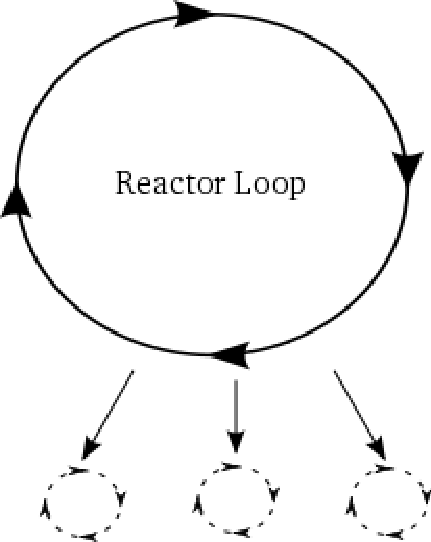
\includegraphics[height=0.3\textheight]{images/reactor-3.pdf}
    \caption{Реактор, вращающий некоторые виртуальные циклы\label{fig:reactor-3}}
\end{center}
\end{figure}


%In this figure we have one big loop, the reactor, and three virtual loops, the individual poetry protocol instances. The big loop spins around and, in so doing, causes the virtual loops to tick over as well, like a set of interlocking gears.
На этом рисунке изображен один большой цикл (реактор) и 
три виртуальных цикла (отдельные экземпляры поэтического протокола). 
Большой цикл крутится и, крутясь, вызывает движение виртуальных 
циклов как будто это множество сцепленных шестеренок.  


\subsection{Беремся за Erlang}

%Erlang, like Python, is a general purpose dynamically typed programming language originally created in the 80′s. Unlike Python, Erlang is functional rather than object-oriented, and has a syntax reminiscent of Prolog, the language in which Erlang was originally implemented. Erlang was designed for building highly reliable distributed telephony systems, and thus Erlang contains extensive networking support.
\href{http://erlang.org/}{Erlang}\footnote[1]{http://erlang.org/} 
подобно Python'у - динамически типизированный язык общего 
назначения, созданный в 80'х. В отличии от Python'а, Erlang больше 
функциональный, чем объектно-ориентированный, и имеет синтаксис, 
напоминающий \href{http://ru.wikipedia.org/wiki/Prolog}{Prolog}\footnote[2]{http://ru.wikipedia.org/wiki/Prolog}, 
язык в котором Erlang был первоначально реализован. 
Erlang был спроектирован для построения высоко 
надежных распределенных телефонных систем, поэтому 
Erlang поддерживает множество вещей, связанных с сетью.


%One of Erlang’s most distinctive features is a concurrency model involving lightweight processes. An Erlang process is neither an operating system process nor an operating system thread. Rather, it is an independently running function inside the Erlang runtime with its own stack. Erlang processes are not lightweight threads because Erlang processes cannot share state (and most data types are immutable anyway, Erlang being a functional programming language). An Erlang process can interact with other Erlang processes only by sending messages, and messages are always, at least conceptually, copied and never shared.
Одна из наиболее заметных особенностей Erlang - это  
параллелизм, основанный на легковесных процессах. 
Процесс в Erlang - это не процесс и не тред в операционной 
системе. Скорее, это независимо выполняющиеся функции 
внутри среды выполнения Erlang'а со своим собственным стеком. 
Erlang процессы это не легковесные треды, поскольку 
Erlang процессы не могут разделять состояние (и большинство 
типов данных неизменяемы (immutable), поскольку Erlang - функциональный 
язык программирования). Процессы Erlang'а могут взаимодействовать с 
другими процессами Erlang'а только отправлением сообщений, и сообщения 
всегда, по меньшей мере концептуально, копируются и никогда не разделяются). 


%So an Erlang program might look like Figure 43:
Таким образом Erlang программа могла бы выглядеть так как рисунке \ref{fig:erlang-1}. 

% fig43
\begin{figure}[h]
\begin{center}
    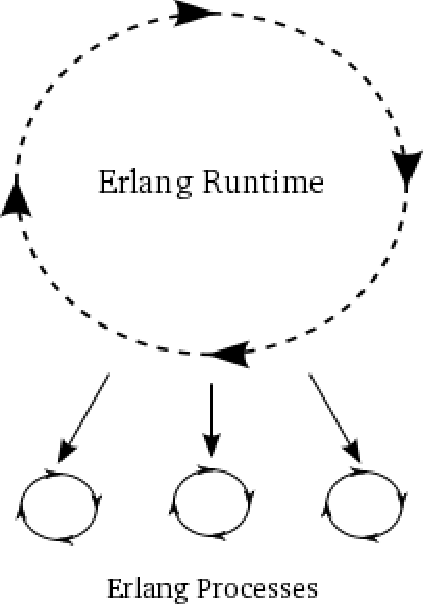
\includegraphics[height=0.3\textheight]{images/erlang-1.pdf}
    \caption{Erlang программа с тремя процессами\label{fig:erlang-1}}
\end{center}
\end{figure}


%In this figure the individual processes have become “real”, since processes are first-class constructs in Erlang, just like objects are in Python. And the runtime has become “virtual”, not because it isn’t there, but because it’s not necessarily a simple loop. The Erlang runtime may be multi-threaded and, as it has to implement a full-blown programming language, it’s in charge of a lot more than handling asynchronous I/O. Furthermore, a language runtime is not so much an extra construct, like the reactor in Twisted, as the medium in which the Erlang processes and code execute.
На этом рисунке отдельные процессы стали <<реальными>>, 
поскольку процессы - конструкции первого класса в Erlang'е, 
подобно объектам в Python'е. Среда исполнения становится 
<<виртуальной>> не потому, что ее нет, а потому что нет 
необходимости в цикле. Среда Erlang может быть многотредовой, и 
она несет ответственность не только за управление асинхронным 
вводом-выводом. Более того, языковая среда - это не дополнительная 
конструкция, подобно реактору в Twisted, это среда, в которой 
Erlang обрабатывает и исполняет код.
 

%So an even better picture of an Erlang program might be Figure 44:
Поэтому, рисунок \ref{fig:erlang-2} лучше соответсвует Erlang программе.

% fig44
\begin{figure}[h]
\begin{center}
    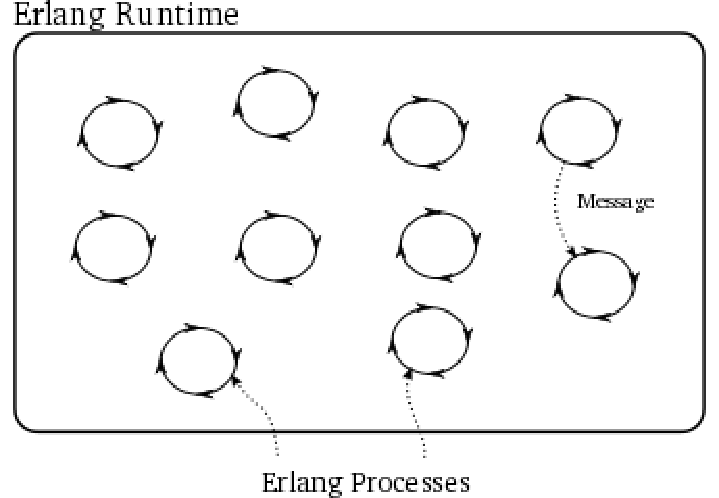
\includegraphics[height=0.3\textheight]{images/erlang-2.pdf}
    \caption{Erlang программа с несколькими процессами\label{fig:erlang-2}}
\end{center}
\end{figure}

%Of course, the Erlang runtime does have to use asynchronous I/O and one or more select loops, because Erlang allows you to create lots of processes. Large Erlang programs can start tens or hundreds of thousands of Erlang processes, so allocating an actual OS thread to each one is simply out of the question. If Erlang is going to allow multiple processes to perform I/O, and still allow other processes to run even if that I/O blocks, then asynchronous I/O will have to be involved.
Конечно, среда Erlang должна использовать асинхронный ввод-вывод и 
один или более select-циклов, поскольку Erlang позволяет создавать 
большое количество процессов. Большие Erlang программы могут 
запустить десятки или сотни Erlang процессов, поэтому создание 
реального потока операционной системы для каждого из них просто вне 
обсуждения. Если Erlang собирается позволить множеству процессов 
выполнить ввод-вывод, и позволить другим процессам выполняться при блокировании 
на вводе-выводе, то понятна необходимость использования асинхронного 
ввода-вывода.

%Note that our picture of an Erlang program has each process running “under its own power”, rather than being spun around by callbacks. And that is very much the case. With the job of the reactor subsumed into the fabric of the Erlang runtime, the callback no longer has a central role to play. What would, in Twisted, be solved by using a callback would, in Erlang, be solved by sending an asynchronous message from one Erlang process to another.
Заметьте, что наш рисунок Erlang программы имеет 
каждый процесс, запущенный <<своей собственной силой>>, а не 
незапущенный обратными вызовами. И это очень важно. 
С задачей реактора, включенной в среду Erlang, 
обратный вызов не имеет больше такого ключевого значения. 
Что решалось бы в Twisted использованием обратных вызовов, 
в Erlang решалось бы отправлением асинхронного сообщения из 
одного Erlang процесса в другой.


\subsection{Erlang поэтический клиент}

%Let’s look at an Erlang poetry client. We’re going to jump straight to a working version instead of building up slowly like we did with Twisted. Again, this isn’t meant as a complete Erlang introduction. But if it piques your interest, we suggest some more in-depth reading at the end of this Part.
Давайте посмотрим на поэтический клиент, написанный 
на Erlang'е. Мы сразу же перейдем к работающей версии 
вместо медленного построения подобно тому, как мы это делали в Twisted. 
И снова напоминаю, что это не полноценное введение в Erlang. 
В конце главы приведены ссылки на дополнительный материал.


%The Erlang client is listed in erlang-client-1/get-poetry. In order to run it you will, of course, need Erlang installed. Here’s the code for the main function, which serves a similar purpose as the main functions in our Python clients:
Исходный код клиента находится в  
\href{http://github.com/jdavisp3/twisted-intro/blob/master/erlang-client-1/get-poetry#L1}{erlang-client-1/get-poetry}. 
Для того, чтобы его запустить, нужно, чтобы был 
установлен \href{http://erlang.org/}{Erlang}. Далее 
код функции 
\href{http://github.com/jdavisp3/twisted-intro/blob/master/erlang-client-1/get-poetry#L96}{main}, 
которая служит тем же целям, что и функция main для 
наших клиентов, написанных на Python'е:

\begin{scriptsize}\begin{verbatim}
main([]) ->
    usage();

main(Args) ->
    Addresses = parse_args(Args),
    Main = self(),
    [erlang:spawn_monitor(fun () -> get_poetry(TaskNum, Addr, Main) end)
     || {TaskNum, Addr} <- enumerate(Addresses)],
    collect_poems(length(Addresses), []).

\end{verbatim}\end{scriptsize}

%If you’ve never seen Prolog or a similar language before then Erlang syntax is going to seem a little odd. But some people say that about Python, too. The main function is defined by two separate clauses, separated by a semicolon. Erlang chooses which clause to run by matching the arguments, so the first clause only runs if we execute the client without providing any command line arguments, and it just prints out a help message. The second clause is where all the action is.
Если вы никогда раньше не видели Prolog или подобный 
язык, то синтаксис Erlang'а вам покажется странным. 
Но многие люди тоже самое говорят о Python'е. В функции  
main определены два отдельных условия, которые разделены  
точкой с запятой. Erlang выбирает какое условие запустить, 
сравнивая аргументы, так что первое условие запускается 
только, если выполняется клиент без  
аргументов командной строки, и он печатает только 
сообщение с помощью (usage). Второе условие - это то, где 
выполняются все действия. 


%Individual statements in an Erlang function are separated by commas, and all functions end with a period. Let’s take each line in the second clause one at a time. The first line is just parsing the command line arguments and binding them to a variable (all variables in Erlang must be capitalized). The second line is using the Erlang self function to get the process ID of the currently running Erlang process (not OS process). Since this is the main function you can kind of think of it as the equivalent of the \_\_main\_\_ module in Python. The third line is the most interesting:
Отдельные операторы в Erlang функции разделяются запятыми, 
и все функции завершаются точкой. Давайте рассмотрим  
каждую строку во втором операторе. Первая строка анализирует  
аргументы командной строки и привязвает их к переменной (все 
переменные в Erlang должны начинаться с заглавной буквы). Вторая строка 
использует функцию \textit{self} Erlang'а для того, чтобы получить 
идентификатор процесса текущего запущенного Erlang процесса (не 
процесса операционной системы). Поскольку это функция main, то 
вы можете подумать о ней как об эквиваленте модуля \_\_main\_\_ в Python'е. 
Третья строчка гораздо интересней: 

\begin{scriptsize}\begin{verbatim}
[erlang:spawn_monitor(fun () -> get_poetry(TaskNum, Addr, Main) end)
     || {TaskNum, Addr} <- enumerate(Addresses)],
\end{verbatim}\end{scriptsize}


%This statement is an Erlang list comprehension, with a syntax similar to that in Python. It is spawning new Erlang processes, one for each poetry server we need to contact. And each process will run the same function (get\_poetry) but with different arguments specific to that server. We also pass the PID of the main process so the new processes can send the poetry back (you generally need the PID of a process to send a message to it).
Этот оператор - список в Erlang'е с синтаксисом, 
похожим на синтаксис в Python'е. Он создает новые Erlang 
процессы, один на каждый поэтический сервер, к которому 
нам надо присоединиться. И каждый процесс запустит одну и ту же 
функцию (\textit{get\_poetry}), но с различными аргументами, 
специфичными только для того сервера. Мы также передаем идентификатор  
главного процесса так, чтобы новые процессы могли отправить 
поэзию обратно (идентификатор процесса нужен, чтобы отправить ему 
сообщение).


%The last statement in main calls the collect\_poems function which waits for the poetry to come back and for the get\_poetry processes to finish. We’ll look at the other functions in a bit, but first you might compare this Erlang main function to the equivalent main in one of our Twisted clients.
Последний оператор в функции main вызывает функцию 
\textit{collect\_poems}, которая ожидает возврата 
поэзии, и завершения процессов \textit{get\_poetry}. 
Мы кратко рассмотрим другие функции, но сначала сравните 
функцию main, написанную на Erlang, с эквивалентом, 
написанным на Twisted для одного из наших поэтических клиентов.



%Now let’s look at the Erlang get\_poetry function. There are actually two functions in our script called get\_poetry. In Erlang, a function is identified by both name and arity, so our script contains two separate functions, get\_poetry/3 and get\_poetry/4 which accept three and four arguments respectively. Here’s get\_poetry/3, which is spawned by main:
Теперь давайте посмотрим на Erlang функцию \textit{get\_poetry}. 
В действительности у нас есть две функции с названием \textit{get\_poetry}. 
В Erlang функция идентифицируется названием и арностью (количеством 
аргументов), так что наш скрипт содержит две разных функции: \textit{get\_poetry/3} 
и \textit{get\_poetry/4}, которые соответственно принимают три и четыре аргумента. 
Далее функция \textit{get\_poetry/3}, которая порождается \textit{main}:

\begin{scriptsize}\begin{verbatim}
get_poetry(Tasknum, Addr, Main) ->
    {Host, Port} = Addr,
    {ok, Socket} = gen_tcp:connect(Host, Port,
                                   [binary, {active, false}, {packet, 0}]),
    get_poetry(Tasknum, Socket, Main, []).
\end{verbatim}\end{scriptsize}


%This function first makes a TCP connection, just like the Twisted client get\_poetry. But then, instead of returning, it proceeds to use that TCP connection by calling get\_poetry/4, listed below:
Эта функция сначала делает TCP соединение, подобно функции 
\textit{get\_poetry} Twisted клиента. Затем, TCP соединение 
продолжает использоваться в вызове \textit{get\_poetry/4}, 
показанной ниже:

\begin{scriptsize}\begin{verbatim}
get_poetry(Tasknum, Socket, Main, Packets) ->
    case gen_tcp:recv(Socket, 0) of
        {ok, Packet} ->
            io:format("Task ~w: got ~w bytes of poetry from ~s\n",
                      [Tasknum, size(Packet), peername(Socket)]),
            get_poetry(Tasknum, Socket, Main, [Packet|Packets]);
        {error, _} ->
            Main ! {poem, list_to_binary(lists:reverse(Packets))}
    end.
\end{verbatim}\end{scriptsize}

%This Erlang function is doing the work of the PoetryProtocol from our Twisted client, except it does so using blocking function calls. The gen\_tcp:recv function waits until some data arrives on the socket (or the socket is closed), however long that might be. But a “blocking” function in Erlang only blocks the process running the function, not the entire Erlang runtime. That TCP socket isn’t really a blocking socket (you can’t make a true blocking socket in pure Erlang code). For each of those Erlang sockets there is, somewhere inside the Erlang runtime, a “real” TCP socket set to non-blocking mode and used as part of a select loop.
Эта Erlang функция выполняет работу \textit{PoetryProtocol} 
из Twisted клиента, за тем исключением, что она продолжает 
использование блокирующих вызовов функций. Функция \textit{gen\_tcp:recv} 
ожидает до тех пор, пока порция данных не прибудет в сокет (или 
сокет не закроется), однако ожидать она может долго. Но "блокирование" 
функции в Erlang только блокирует процесс, запускающий функцию, а не всю 
среду Erlang. Рассмотренный TCP сокет в действительности не блокирующийся 
сокет (вы не можете создать реально блокирующийся сокет, используя чистый Erlang). 
Для каждого из Erlang сокетов существует где-то внутри среды Erlang 
<<настоящий>> TCP сокет, установленный в неблокирующее состояние и использованный 
как часть select-цикла.


%But the Erlang process doesn’t have to know about any of that. It just just waits for some data to arrive and, if it blocks, some other Erlang process can run instead. And even if a process never blocks, the Erlang runtime is free to switch execution from that process to another at any time. In other words, Erlang has a non-cooperative concurrency model.
Но Erlang процесс не должен про все это знать. Он 
просто ожидает некоторых данных, и если он блокируется, 
то выполняется другой Erlang процесс. И даже, если 
процесс никогда не блокируется, среда Erlang в произвольный 
момент времени может переключиться 
на выполнение другого процесса. Другими словами, Erlang основано 
на некооперативной модели параллелизма (non-cooperative concurrency model).  
  

%Notice that get\_poetry/4, after receiving a bit of poem, proceeds by recursively calling itself. To an imperative language programmer this might seem like a recipe for running out of memory, but the Erlang compiler can optimize “tail” calls (function calls that are the last statement in a function) into loops. And this highlights another curious parallel between the Erlang and Twisted clients. In the Twisted client, the “virtual” loops are created by the reactor calling the same function (dataReceived) over and over again. And in the Erlang client, the “real” processes running (get\_poetry/4) form loops by calling themselves over and over again via tail-call optimization. How about that.

Заметьте, что \textit{get\_poetry/4} после получения порции поэмы 
продолжает рекурсивно себя вызывать. В императивном языке это подобно 
рецепту для переполнения стека и выхода за пределы доступной памяти, но 
Erlang компилятор может оптимизировать хвостовые вызовы (функциональные 
вызовы, которые являются последними операторами в функции) и превращать их 
в циклы. И это подчеркивает еще одну любопытную параллель между Erlang и 
Twisted клиентами. В Twisted клиенте, <<виртуальные>> циклы создаются 
реактором многократным вызовом одной и той же функции (dataReceived) снова и снова. 
А в Erlang клиенте <<действительные>> процессы (\textit{get\_poetry/4}) 
образуют цикл путем вызова самих себя снова и снова с использованием 
\href{http://stackoverflow.com/questions/310974/what-is-tail-call-optimization}{оптимизации хвостового вызова}.



%If the connection is closed, the last thing get\_poetry does is send the poem to the main process. That also ends the process that get\_poetry is running, as there is nothing left for it to do.
Если соединение закрывается, последнее, что делает \textit{get\_poetry} - 
это отправляет поэму обратно процессу main. Это также завершает выполнение 
\textit{get\_poetry}, поскольку делать уже нечего.


%The remaining key function in our Erlang client is collect\_poems:
Оставшаяся ключевая функция нашего Erlang клиента это 
\href{http://github.com/jdavisp3/twisted-intro/blob/master/erlang-client-1/get-poetry#L58}{collect\_poems}:

\begin{scriptsize}\begin{verbatim}
collect_poems(0, Poems) ->
    [io:format("~s\n", [P]) || P <- Poems];
collect_poems(N, Poems) ->
    receive
        {'DOWN', _, _, _, _} ->
            collect_poems(N-1, Poems);
        {poem, Poem} ->
            collect_poems(N, [Poem|Poems])
    end.
\end{verbatim}\end{scriptsize}


%This function is run by the main process and, like get\_poetry, it recursively loops on itself. It also blocks. The receive statement tells the process to wait for a message to arrive that matches one of the given patterns, and then extract the message from its “mailbox”.
Эта функция запускается процессом main и, подобно \textit{get\_poetry}, 
она рекурсивно вызывает саму себя. Она также блокируется. Оператор \textit{receive} 
говорит процессу ждать прибытия сообщения, которое соответсвует 
одному из заданных шаблонов, затем извлечь сообщение из его слота (mailbox).


%The collect\_poems function waits for two kinds of messages: poems and “DOWN” notifications. The latter is a message sent to the main process when one of the get\_poetry processes dies for any reason (this is the monitor part of spawn\_monitor). By counting DOWN messages, we know when all the poetry has finished. The former is a message from one of the get\_poetry processes containing one complete poem.
Функция \textit{collect\_poems} ожидает двух видов 
сообщений: поэм и уведомлений типа <<DOWN>>. Уведомление типа <<DOWN>> - сообщение, 
посылаемое процессу main, когда один из процессов \textit{get\_poetry} 
по какой-то причине обрушился (это часть мониторига \textit{spawn\_monitor}). 
Подсчитывая "DOWN" сообщения, мы узнаем, когда вся поэзия завершилась. 
Шаблон - сообщение от одного из \textit{get\_poetry} процессов, 
содержащих одну завершенную поэму.

%Ok, let’s take the Erlang client out for a spin. First start up three slow poetry servers:
Хорошо, давайте  запустим Erlang клиент. Сначала запустим три медленных 
поэтических сервера:

\begin{scriptsize}\begin{verbatim}
python blocking-server/slowpoetry.py --port 10001 poetry/fascination.txt
python blocking-server/slowpoetry.py --port 10002 poetry/science.txt
python blocking-server/slowpoetry.py --port 10003 poetry/ecstasy.txt --num-bytes 30
\end{verbatim}\end{scriptsize}


%Now we can run the Erlang client, which has a similar command-line syntax as the Python clients. If you are on a Linux or other UNIX-like system, then you should be able to run the client directly (assuming you have Erlang installed and available in your PATH). On Windows you will probably need to run the escript program, with the path to th Erlang client as the first argument (with the remaining arguments for the Erlang client itself).
Теперь вы можете запустить Erlang клиент, который 
имеет похожий синтаксис командной строки, что и 
Python клиенты. Если вы используете Linux или другую 
UNIX-подобную систему, то вам следует запустить 
клиент напрямую (предполагается, что вы установили 
Erlang и он доступен по вашей переменной окружения \textit{PATH}). 
В Windows вам нужно будет запустить программу escript c путем к 
Erlang клиенту в качестве первого аргумента (и с остальными 
аргументами для самого Erlang клиента).

\begin{scriptsize}\begin{verbatim}
./erlang-client-1/get-poetry 10001 10002 10003
\end{verbatim}\end{scriptsize}

%After that you should see output like this:
После запуска вы увидите примерно следующее:

\begin{scriptsize}\begin{verbatim}
Task 3: got 30 bytes of poetry from 127:0:0:1:10003
Task 2: got 10 bytes of poetry from 127:0:0:1:10002
Task 1: got 10 bytes of poetry from 127:0:0:1:10001
...
\end{verbatim}\end{scriptsize}

%This is just like one of our earlier Python clients where we print a message for each little bit of poetry we get. When all the poems have finished the client should print out the complete text of each one. Notice the client is switching back and forth between all the servers depending on which one has some poetry to send.
Это похоже на вывод одного из наших ранних Python 
клиентов, где вы печатаем сообщение для каждого полученного небольшого 
куска поэзии. Когда все поэмы скачаются, клиент напишет 
полный текст каждой из поэм. Заметьте, что клиент переключается 
между всеми серверами взависимости от того, какой сервер отправил кусок поэзии.

% fig45
\begin{figure}[h]
\begin{center}
    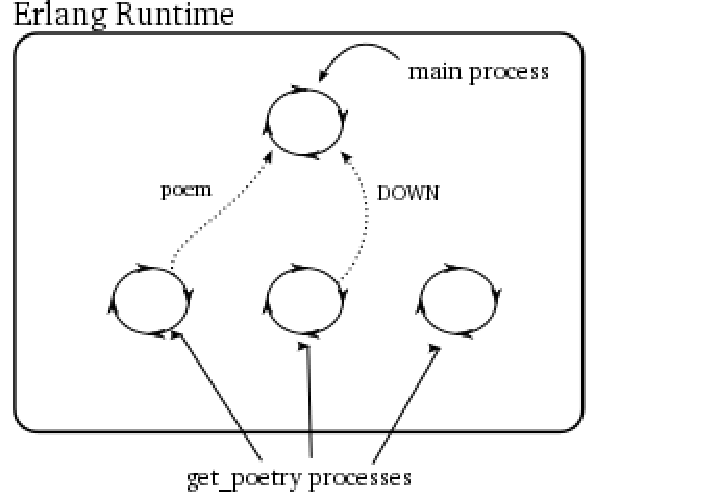
\includegraphics[width=0.5\textwidth]{images/erlang-3.pdf}
    \caption{Поэтический клиент на Erlang\label{fig:erlang-3}}
\end{center}
\end{figure}


%This figure shows three get\_poetry processes (one per server) and one main process. You can also see the messages that flow from the poetry processes to main process.
На рисунке \ref{fig:erlang-3}  изображено три процесса \textit{get\_poetry} (один 
на каждый сервер) и один main процесс. Вы также можете увидеть 
сообщения, идущие от поэтических процессов к main процессу. 


%So what happens if one of those servers is down? Let’s try it:
Так что же случается, если один из этих серверов не доступен? 
Давайте попробуем следующее:
\begin{scriptsize}\begin{verbatim}
./erlang-client-1/get-poetry 10001 10005
\end{verbatim}\end{scriptsize}


%The above command contains one active port (assuming you left all the earlier poetry servers running) and one inactive port (assuming you aren’t running any server on port 10005). And we get some output like this:
Команда выше содержит один действующий порт (предполагается, 
что оставили все ранее запущенные поэтические серверы), и 
один - недействующий (предполагается, что вы не запустили 
никакого сервера на порту 10005). И мы получаем некоторый вывод 
подобный приведенному ниже:

\begin{scriptsize}\begin{verbatim}
Task 1: got 10 bytes of poetry from 127:0:0:1:10001

=ERROR REPORT==== 25-Sep-2010::21:02:10 ===
Error in process <0.33.0> with exit value: {{badmatch,{error,econnrefused}},[{erl_eval,expr,3}]}

Task 1: got 10 bytes of poetry from 127:0:0:1:10001
Task 1: got 10 bytes of poetry from 127:0:0:1:10001
...
\end{verbatim}\end{scriptsize}

%And eventually the client finishes downloading the poem from the active server, prints out the poem, and exits. So how did the main function know that both processes were done? That error message is the clue. The error happens when get\_poetry tries to connect to the server and gets a connection refused error instead of the expected value ({ok, Socket}). The resulting exception is called badmatch because Erlang “assignment” statements are really pattern-matching operations.
Под конец клиент завершает скачивание поэмы из 
действующего сервера, выводит поэму и выходит. 
Так как же функция main узнает, что оба процесса 
завершились? Сообщение об ошибке выше - подсказка. 
Ошибка происходит, когда \textit{get\_poetry} пытается 
присоединиться к серверу и получает ошибку отказа в 
соединении (<<connection refused>>) вместо ожидаемого значения ({ok, Socket}). 
Результирующее исключение называется ошибка сопоставления, 
поскольку операторы <<присваивания>> в Erlang являются в 
действительности операторами сопоставления шаблону.
  

%An unhandled exception in an Erlang process causes the process to “crash”, which means the process stops running and all of its resources are garbage collected. But the main process, which is monitoring all of the get\_poetry processes, will receive a DOWN message when any of those processes stops running for any reason. And thus our client exits when it should instead of running forever.
Необработанное исключение в Erlang процессе вызывает 
<<разрушение>> процесса, что означает, что процесс останавливает 
выполнение и все его ресурсы утилизируются сборщиком мусора. 
Но процесс main, который контролирует все \textit{get\_poetry} 
процессы, будет получать все DOWN-сообщения, когда любые из 
этих процессов завершат выполнение по какой-то причине. 
Таким образом, наш клиент завершается, а не выполняется бесконечно. 

\subsection{Обсуждение}

%Let’s take stock of some of the parallels between the Twisted and Erlang clients:
Давайте выявим некоторые параллели между Twisted и Erlang клиентами:

\begin{enumerate}

%   1. Both clients connect (or try to connect) to all the poetry servers at once.
\item Оба клиента соединяются (или пытаются соединиться) со всеми поэтическими серверами одновременно.

%   2. Both clients receive data from the servers as soon as it comes in, regardless of which server delivers the data.
\item Оба клиента получают данные из серверов как только они приходят, 
независимо от того, какие сервера доставили данные.

%   3. Both clients process the poetry in little bits, and thus have to save the portion of the poems received thus far.
\item Оба клиента обрабатывают поэзию маленькими порциями, поэтому должны 
сохранять порцию полученных поэм.

%   4. Both clients create an “object” (either a Python object or an Erlang process) to handle all the work for one particular server.
\item Оба клиента создают "объект" (либо Python объект, либо Erlang процесс) для 
работы с одним определенным сервером.

%   5. Both clients have to carefully determine when all the poetry has finished, regardless of whether a particular download succeeded or failed.
\item Оба клиента должны аккуратно определять, когда вся поэзия скачалась, 
независимо от того успешно или неуспешно произошло определенное скачивание.

\end{enumerate}


%And finally, the main functions in both clients asynchronously receive poems and “task done” notifications. In the Twisted client this information is delivered via a Deferred while the Erlang client receives inter-process messages.
И наконец, функции main в обоих клиентах асинхронно получают 
поэмы и уведомления о завершении задачи. В Twisted клиенте эта информация 
доставляется через Deferred, в то время как Erlang получает межпроцессорные 
сообщения (inter-process messages).
 

%Notice how similar both clients are, in both their overall strategy and the structure of their code. The mechanics are a bit different, with objects, deferreds, and callbacks on the one hand and processes and messages on the other. But the high-level mental models of both clients are quite similar, and it’s pretty easy to move from one to the other once you are familiar with both.
Заметьте как похожи оба клиента, в своих общих стратегиях и 
структуре их кода. Механизмы немного отличаются: 
с объектами, deferred'ми, callback'ми с одной стороны; 
процессами и сообщениями с другой стороны. Но высокоуровневые 
модели обоих клиентов практически одинаковые, и достаточно 
просто понять один, зная другой.


%Even the reactor pattern reappears in the Erlang client in miniaturized form. Each Erlang process in our poetry client eventually turns into a recursive loop that:
Даже шаблон проектирования reactor появляется в миниатюре в Erlang клиенте. 
Каждый Erlang процесс в нашем поэтическом клиенте превращается в 
рекурсивный цикл, который:

\begin{enumerate}

%   1. Waits for something to happen (a bit of poetry comes in, a poem is delivered, another process finishes), and
\item Ожидает что что-то произойдет (пришел кусок поэзии, поэма доставлена, 
другой процесс завершился).

%   2. Takes some appropriate action.
\item Производит определенное действие.

\end{enumerate}


%You can think of an Erlang program as a big collection of little reactors, each spinning around and occasionally sending a message to another little reactor (which will process that message as just another event).
Вы можете думать об Erlang программе как о большой коллекции маленьких 
реакторов, каждый из которых выполняется в цикле и отправляет сообщение 
другому маленькому реактору (который обработает это сообщение как еще одно событие).


%And if you delve deeper into Erlang you will find callbacks making an appearance. The Erlang gen\_server process is a generic reactor loop that you “instantiate” by providing a fixed set of callback functions, a pattern repeated elsewhere in the Erlang system.
И если вы копнете глубже в Erlang, вы обнаружите 
обратные вызовы. Erlang процесс \textit{gen\_server} - это 
общий цикл реактора, экземпляр которого вы создаете, 
предоставляя фиксированное множество callback-функций, а также это 
шаблон, повторямый везде в Erlang системе.

%So if, having learned Twisted, you ever decide to give Erlang a try I think you will find yourself in familiar mental territory.
Поэтому, изучив Twisted, вы даже можете решить попробовать Erlang и, 
возможно, обнаружите близкую к вам среду. 
 

\subsection{Для дальнейшего ознакомления}

%In this Part we’ve focused on the similarities between Twisted and Erlang, but there are of course many differences. One particularly unique feature of Erlang is its approach to error handling. A large Erlang program is structured as a tree of processes, with “supervisors” in the higher branches and “workers” in the leaves. And if a worker process crashes, a supervisor process will notice and take some action (typically restarting the failed worker).
В этой главе мы сфокусировались на схожих стороных между 
Twisted и Erlang, но есть много отличий. Одно особенное 
уникальное свойство Erlang - это его метод управления ошибками. 
Большие Erlang программы структурированы как дерево 
процессов, с <<супервизорами>> (<<supervisors>>)  в ветвях и <<рабочими>> (<<workers>>) 
в листьях. Если рабочий процесс рушится, процесс-супервизор сообщит об этом 
и сделать некоторые дейтсвия (обычно - перезапустит рухнувший рабочий процесс).


%If you are interested in learning more Erlang then you are in luck. Several Erlang books have either been published recently, or will be published shortly:
Если вас заинтересовало изучениие Erlang'а, то вы можете почитать приведенные 
далее книги по Erlang'у, которые были недавно опубликованы 
или которые скоро будут опубликованы: 

\begin{itemize}

%    * Programming Erlang — written by one of Erlang’s inventors. A great introduction to the language.
\item \href{http://www.amazon.com/exec/obidos/ASIN/193435600X/krondonet-20}{Programming Erlang}\footnote[1]{http://www.amazon.com/exec/obidos/ASIN/193435600X/krondonet-20}. Книга написана одним из создателей Erlang'а. 
Прекрасное введение в язык.

%    * Erlang Programming — this complements the Armstrong book and goes into more detail in several key areas.
\item \href{http://www.amazon.com/exec/obidos/ASIN/0596518188/krondonet-20}{Erlang Programming}\footnote[2]{http://www.amazon.com/exec/obidos/ASIN/0596518188/krondonet-20}. Это дополнение к книге Армстронга и 
содержит больше деталей по нескольким ключевым темам. 

%    * Erlang and OTP in Action — this hasn’t been published yet, but I am eagerly awaiting my copy. Neither of the first two books really addresses OTP, the Erlang framework for building large apps. Full disclosure: two of the authors are friends of mine.
\item \href{http://www.amazon.com/exec/obidos/ASIN/1933988789/krondonet-20}{Erlang and OTP in Action}\footnote[3]{http://www.amazon.com/exec/obidos/ASIN/1933988789/krondonet-20}. Эта книга, возможно еще не опубликована. В ней, в отличии 
от двух предыдущих, рассматривается OTP: Erlang система для построения больших приложений.

\end{itemize}


%Well that’s it for Erlang. In the next Part we will look at Haskell, another functional language with a very different feel from either Python or Erlang. Nevertheless, we shall endeavor to find some common ground.
На этом мы завершаем рассмотрение Erlang'а. В следующей главе мы 
посмотрим на Haskell, еще один функциональный язык, очень отличающийся 
от Python'а и Erlang'а. Тем не менее, мы попытаемся найти что-то общее.


\subsection{Упражнения для особо мотивированных}

\begin{enumerate}

%   1. Go through the Erlang and Python clients and identify where they are similar and where they differ. How do they each handle errors (like a failure to connect to a poetry server)?
\item Просмотрите Erlang и Python клиенты и идентифицируйте, где они 
похожи, и где отличаются. Как каждый из них обрабатывает ошибки (например, ошибкой 
соединения с поэтическим сервером)? 

%   2. Simplify the Erlang client so it no longer prints out each bit of poetry that comes in (so you don’t need to keep track of task numbers either).
\item Упроситите Erlang клиент так, чтобы он больше не 
печатал каждый полученный кусок поэзии (также вам не нужно хранить номера задач).

%   3. Modify the Erlang client to measure the time it takes to download each poem.
\item Модифицируйте Erlang клиент, чтобы замерить время, которое он 
тратит на скачивание каждой поэмы.

%   4. Modify the Erlang client to print out the poems in the same order as they were given on the command line.
\item Модифицируйте Erlang клиент, чтобы он выводил поэмы в том же 
порядке, в котором они были даны в командной строке. 

%   5. Modify the Erlang client to print out a more readable error message when we can’t connect to a poetry server.
\item Модифицируйте Erlang клиент, чтобы он вывол более читабельные 
сообщения с ошибкой, когда мы не можем соединиться с поэтическим сервером.

%   6. Write Erlang versions of the poetry servers we made with Twisted.
\item Напишите Erlang версии  поэтических серверов, которые мы сделали с помощью Twisted.

\end{enumerate}


